\chapter{Background}

\section{The Maritime Connectivity Platform}
The Maritime Connectivity Platform (MCP), formally known as the Maritime Cloud, is a platform, developed by EfficienSea2~\cite{efficienSea2}, which is led by the Danish Maritime Authority. 
MCP is a communication framework, that is to ensure efficient, reliable and secure communication, and exchange of information in the maritime sector.
The goal of the platform is to connect maritime stakeholders with maritime information services.
\begin{figure}
  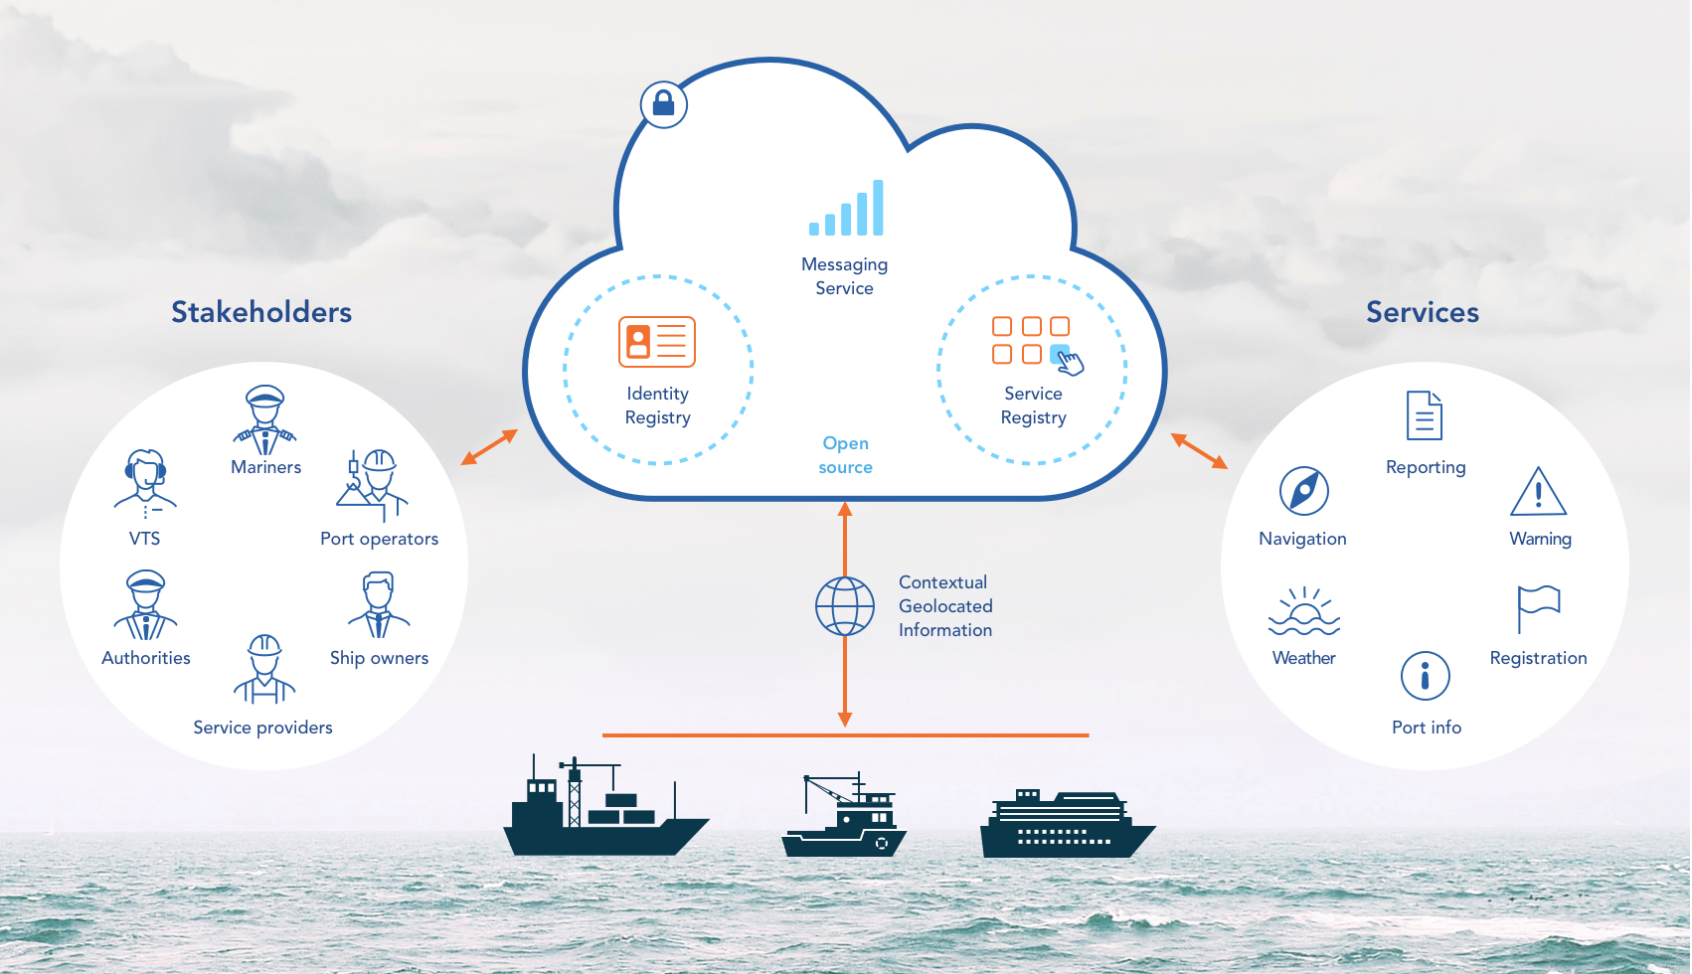
\includegraphics[width=1\textwidth]{figures/MCPStructure}
  \caption{Diagram, describing the structure of MCP~\cite{efficienSea2}.}
  \label{fig:MCPStruct}
\end{figure}\noindent
A high-level diagram, describing the structure of the MCP can be seen in Figure~\ref{fig:MCPStruct}. Here it is shown that maritime stakeholders are connected with the maritime services through the Identity Registry, the Service Registry and the Messaging Service.

\subsection{Identity Registry}
Here the relevant information regarding maritime stakeholders are stored. This information needs to be authorized and stored at a safe location in order for the security of the MCP to be sufficient. The Identity Registry on the MCP is equivalent to the Central Person Registry of a country. The Identity Registry is vital to the MCP, in that it ensures the solution's authenticity, integrity, and confidentiality. Maritime stakeholders are, through the Identity Registry, provided with a single login to all Maritime Services~\cite{efficienSea2}.
\subsection{Service Registry}
What the Identity Registry provides for the Maritime Stakeholders, the Service Registry provides for the Maritime Services. Here all Maritime Services are registered and stored. The Service Registry provides both commercial and non-commercial, as well as authorized and non-authorized services, either free of charge or for a fee. The Service Registry is comparable with the App Store or Google Play, in that it distributes services of all kinds to registered users~\cite{efficienSea2}.
\subsection{Messaging Service}
The messaging service in the MCP, enables the exchange of information across the different platforms, thereby linking their systems to each other. The messaging service accounts for the available means of communication, as well as the geographical coordinates of the destination and origin of the information, being sent~\cite{efficienSea2}.

\section{Parsing}
Parsing is a widely known tool in computer science. The term expresses a function, taking a string of input, from which it yields a parse tree that it constructs when applying the specific parser logic upon the input string. The parser performs a lexical analysis, meaning that it converts sections of the string to tokens, that are ultimately easier to handle by an interpreter. When using Erlang to define parsers, a library family known as parser combinators is very popular, in that it allows the programmer to embed domain specific language directly into the parser. The concept of combinatory parsing is using one or more of these libraries of higher-order functions, known as parser combinators. Parser combinators take in parsers of any kind imaginable as input and returns a new set of parsers as an output.
\newpage
\subsection{Monadic Parsing}
Before 1995, implementation of top-down parsing, using parser combinators ran in and used both exponential time and space complexity, when applied to ambiguous, context free grammars. At that time Frost and Szydlowski demonstrated that memoization can enhance parser combinators in order to optimize time complexity to polynomial~\cite{memoization}. One year later through the use of monads, Haskell-specific parser combinators were reconstructed by Frost which introduced systematic and correct threading of memoization throughout execution.

\section{Interpretation}
In solutions, utilizing parsers, an interpreter is often introduced to handle the result that the parser returns, and for this reason, interpreters share the same syntax that is used in their corresponding parsers. The job of an interpreter is to execute the parsed commands, and therefor their implementation can vary to an even higher extend than that of a parser. Often-times a parser-interpreter combination is used to identify, generate, as well as execute domain-specific languages. Since automatic utilization of domain-specific language is an integral part of the problem-statement, using a parser- and interpreter-combination is straightforward to the solution.

\section{Property-Based Testing}

Property-based testing, also known as Automation Testing, is the principle of testing properties of code, rather than instances, as is done in manual unit testing. Unit tests are fast and easy to set up and execute, however, in most instances they only provide coverage to a certain degree.

\begin{figure}[h]
  \centering
  \begin{lstlisting}
import Test.QuickCheck
import Data.List

qsort :: Ord a => [a] -> [a]
qsort []     = []
qsort (x:xs) = qsort lhs ++ [x] ++ qsort rhs
    where lhs = filter  (< x) xs
          rhs = filter (>= x) xs

prop_idempotent xs = qsort (qsort xs) == qsort xs
  \end{lstlisting}
  \caption{Example of Property-Based Testing~\cite{realWorldHaskell11}}.
  \label{fig:pbtEx}
\end{figure}\ \\

\noindent
Depending on the complexity of the given program, most programmers can come up with tests, covering most of the given program, however, many edge-cases are unintuitive and would require extensive testing to discover manually. Property-based testing solves this problem by setting up test cases that take into account mathematical models, describing the desired behavior of the code. Once such a test case has been created, semi-random execution instances can be run to the point of literal exhaustion, and thus a relatively small program can test for thousands of occurrences at once.

An example of this can be seen in Listing~\ref{fig:pbtEx}, which describes a snippet of Haskell quicksort code. A property of quicksort is that a list, sorted once is equivalent to that list, sorted twice, and this is what the function \lstinline{prop_idempotent} validates.

\section{Model-Based Testing}

The principle of Model-based testing is to check behavior of software against predictions made by a model. Behavior can be described in a variety of manners, including data flow, control flow, dependencies, decision trees/cycles, and state transition machines. Model-based testing is good at describing the behavior of a system, when it reacts to a specific action, which is determined by another specific model. Using this technique, the behavior of a system can easily be determined and validated. Currently there are two main types of model-based testing-techniques:

\begin{description}
  \item[Serial model building- and testing],
  is a way of implementing model-based testing and involves predefined models, upon which a number of tests are executed. Creating the tests manually ahead of execution allows the tester to implement an additional layer of complexity to the created models. Furthermore, implementing this strain of model-based testing allows for custom-tailored testing, suited to fit issues, unique to the corresponding model. Depending on the amount of models, this is, however, a significantly slower process than the alternative, in that each model requires a similar amount of time to construct. Depending on the developer, as well as the implementation techniques of models, a relatively high leaning curve may be introduced, leading to exclusions of parties, not qualified to take on this task. 
  Figure~\ref{fig:serialMBT} provides a high-level diagram, describing this principle, using arbitrary measurement units of time consumption, skill level, and model complexity along its $y$-axis, and amount of models along its $x$-axis. \newpage
  \begin{figure}[h]
    \centering
    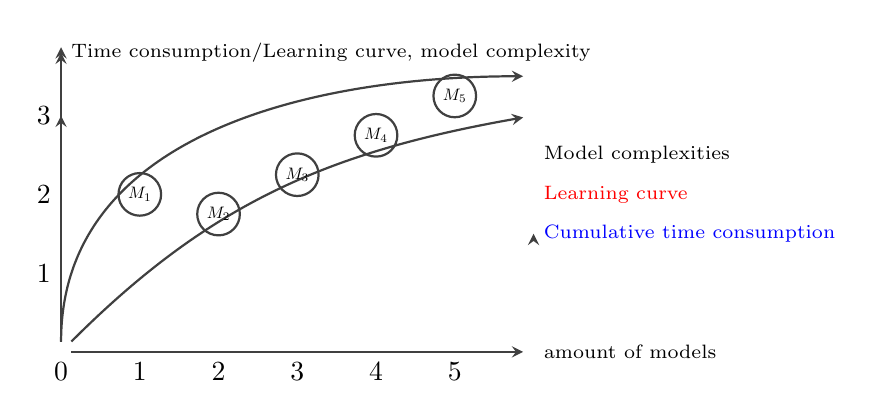
\begin{tikzpicture}[thick]
      % horizontal and vertival axis
      \node (Z) at (0,0) {};
      \node (X) at (6,0) {};
      \node (Y) at (0,4) {};

      \path [] (Z) edge (X);
      \path [] (Z) edge (Y);

      % horizontal labels
      \draw (0,0) node[anchor=north]  {0}
            (1,0) node[anchor=north]  {1}
            (2,0) node[anchor=north]  {2}
            (3,0) node[anchor=north]  {3}
            (4,0) node[anchor=north]  {4}
            (5,0) node[anchor=north]  {5}

      % vertical labels
            (0,1) node[anchor=east] {1}
            (0,2) node[anchor=east] {2}
            (0,3) node[anchor=east] {3};
      
      \node (L) at (6,3.5) {};
      \node (T) at (6,3) {};

      \path [red, out=90, in=180] (Z) edge (L);
      \path [blue,out=45, in=190] (Z) edge (T);

      \draw (6,2.5) node[anchor=west] {\scriptsize\color{black} Model complexities}
            (6,2)   node[anchor=west] {\scriptsize\color{red}   Learning curve}
            (6,1.5) node[anchor=west] {\scriptsize\color{blue}  Cumulative time consumption};
      
      \draw (0,3.8) node[anchor=west] {\scriptsize Time consumption/Learning curve, model complexity};
      \draw (X)     node[anchor=west] {\scriptsize amount of models};

      \node (M1)  [circle,  draw, scale=0.6] at (1,2)   {$M_1$};
      \node (M2)  [circle,  draw, scale=0.6] at (2,1.75)  {$M_2$};
      \node (M3)  [circle,  draw, scale=0.6] at (3,2.25)  {$M_3$};
      \node (M4)  [circle,  draw, scale=0.6] at (4,2.75)  {$M_4$};
      \node (M5)  [circle,  draw, scale=0.6] at (5,3.25)  {$M_5$};
    \end{tikzpicture}
    \caption{Time consumption and learning curve of serial model building and testing.}
    \label{fig:serialMBT}
  \end{figure}\ \\
  Figure~\ref{fig:serialMBT} shows the time consumption increasing for every model built, while the learning curve initiates very steeply, however diverges, as the creator of the models learns the used techniques. 
  \item[Sequential model building- and testing],
  is a way of implementing model-based testing, that involves on-the-fly model creation- and testing. Here, a program is designed to take in arguments, describing different model behaviors, upon the basis of which the program tests the models immediately after they are generated. Compared with the implementation described above, this technique scales to a much better degree, as the program will only need to be written once in order to create a virtually infinite amount of models. 
  Input, containing all necessary information that would otherwise be entered manually is, however, still needed, and thus scalability is not completely eliminated. 

  Figure~\ref{fig:sequenceMBT} provides a high-level diagram, describing this principle, using arbitrary measurement units of time consumption, skill level, and model complexity along its $y$-axis, and amount of models along its $x$-axis.
  \begin{figure}[h]
    \centering
    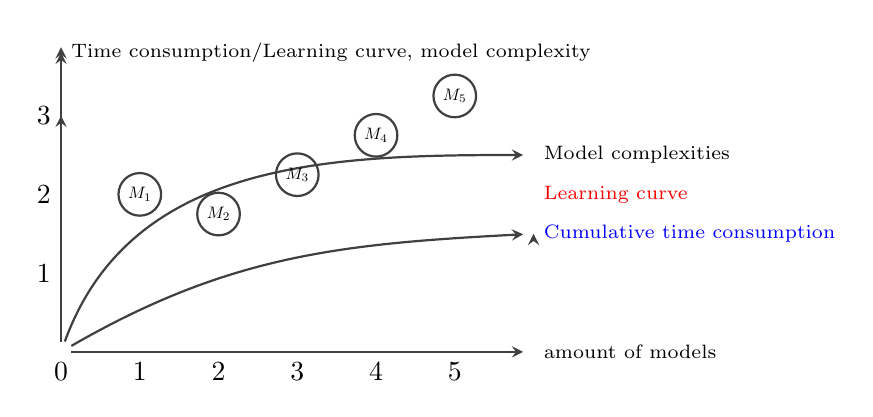
\begin{tikzpicture}[thick]
      % horizontal and vertival axis
      \node (Z) at (0,0) {};
      \node (X) at (6,0) {};
      \node (Y) at (0,4) {};

      \path [] (Z) edge (X);
      \path [] (Z) edge (Y);

      % horizontal labels
      \draw (0,0) node[anchor=north]  {0}
          (1,0) node[anchor=north]  {1}
          (2,0) node[anchor=north]  {2}
          (3,0) node[anchor=north]  {3}
          (4,0) node[anchor=north]  {4}
          (5,0) node[anchor=north]  {5}

      % vertical labels
          (0,1) node[anchor=east] {1}
          (0,2) node[anchor=east] {2}
          (0,3) node[anchor=east] {3};
      
      \node (L) at (6,2.5){};
      \node (T) at (6,1.5){};

      \path [red, out=70, in=180] (Z) edge (L);
      \path [blue,out=30, in=183] (Z) edge (T);

      \draw (6,2.5) node[anchor=west] {\scriptsize\color{black} Model complexities}
          (6,2) node[anchor=west] {\scriptsize\color{red}   Learning curve}
          (6,1.5) node[anchor=west] {\scriptsize\color{blue}  Cumulative time consumption};
      
      \draw (0,3.8) node[anchor=west] {\scriptsize Time consumption/Learning curve, model complexity};
      \draw (X)     node[anchor=west] {\scriptsize amount of models};

      \node (M1)  [circle,  draw, scale=0.6] at (1,2)   {$M_1$};
      \node (M2)  [circle,  draw, scale=0.6] at (2,1.75)  {$M_2$};
      \node (M3)  [circle,  draw, scale=0.6] at (3,2.25)  {$M_3$};
      \node (M4)  [circle,  draw, scale=0.6] at (4,2.75)  {$M_4$};
      \node (M5)  [circle,  draw, scale=0.6] at (5,3.25)  {$M_5$};
    \end{tikzpicture}
    \caption{Time consumption and learning curve of sequential model building and testing.}
    \label{fig:sequenceMBT}
  \end{figure}\\
  Like Figure~\ref{fig:serialMBT}, Figure~\ref{fig:sequenceMBT} introduces a learning curve, as the user will need to become familiar with the input needing to be specified, in order for the sequential model creation to start, however, this is severely more gradual, while also featuring a lower end-point than the one seen in Figure~\ref{fig:serialMBT}. The cumulative time consumption is also lower, compared to serial model building, due to the fact that this process will run semi-automatically, only needing input from a user, before handling all building-related tasks.
\end{description}
\newpage
\subsection{Finite State Machines (FSM)}
A finite state machine is, as the name suggests, a mathematical machine, consisting of a collection of states and actions. An arbitrary FSM has a start state along with a collection of states that are accessed through various status- and/or input-combinations. An example of this can be seen in Figure~\ref{fig:fsmEx}, which describes the flow of a turnstile, which allows for one pass through, after which it prompts for a coin before allowing another pass through.

\begin{figure}[h]
  \centering
  \begin{tikzpicture}[->,>=stealth', node distance=3.5 cm, thick]
    \tikzstyle{every state}=[rectangle,
                       draw=gray,
                       rounded corners,
                       rectangle,
                       top color=white,
                       bottom color=gray!50]
    \tikzstyle{every path}=[->,gray!150,>=stealth,text=black]

    \node[state, initial] (A) []      {Locked};
    \node[state]      (B) [right of=A]{Unlocked};

    \path (A) edge  [bend left, above]  node  {Insert Coin} (B)
          edge  [loop above,above]  node  {Pass Through}  (A)
        (B) edge  [loop above,above]  node  {Insert Coin} (B)
          edge  [bend left, below]  node  {Pass Through}  (A);
  \end{tikzpicture}
  \caption{Example of a finite state machine, describing a turnstile. Furthermore, this figure describes Table~\ref{tab:fsmEx}.}
  \label{fig:fsmEx}
\end{figure}
In addition to describing the concept of states in a FSM, Figure~\ref{fig:fsmEx} and Table~\ref{tab:fsmEx} also displays a collection of actions. An action is an operation that is performed along with a corresponding state, which can potentially change that state. The described case, features the two actions `Insert Coin' and `Pass Through'. The action `Insert Coin' alters the state of the turnstile, only if performed when the state of the turnstile is `Locked', as it is not possible to unlock an already unlocked lock. Similarly, the action `Pass Through' only changes the state if the turnstile is in its unlocked state before performing the action, as passing through a locked turnstile is not possible.
\newpage
\noindent
Table~\ref{tab:fsmEx}, seen below displays the relationships between the actions, states and output, produced when interacting with the turnstile, using its intended functionality. The table features the four columns, with `State' describing the state before execution of the `Action' column. `Next State' describes the state after the action has taken effect, and the `Output' column describes the flow of events, leading to the next state. Note that the Output column features event flows that do \tit{not} lead to a change in state, as well as outcomes that do.
\begin{table}[h]
  \centering
  \begin{tabular}{l|l|l|l}\toprule
    State   & Action    & Next State& Output \\ \midrule
    Locked    & Insert Coin & Unlocked  & \colorbox{green}{Unlocks turnstile, allowing passage.} \\
    Locked    & Push      & Locked  & \colorbox{red}{Blocks passage.} \\
    Unlocked  & Insert Coin & Unlocked  & \colorbox{green}{Returns coin.} \\
    Unlocked  & Push      & Locked  & \colorbox{red}{Allows passage, locks.} \\ \bottomrule
  \end{tabular}
  \caption{Example of a finite state machine, describing a turnstile. Furthermore, this table describes Figure~\ref{fig:fsmEx}.}
  \label{tab:fsmEx}
\end{table}